\documentclass[11pt,a4paper]{article}

% ============================================
% PACKAGES
% ============================================
\usepackage[utf8]{inputenc}
\usepackage[T1]{fontenc}
\usepackage{lmodern}
\usepackage[margin=2.5cm]{geometry}
\usepackage{graphicx}
\usepackage{booktabs}
\usepackage{tabularx}
\usepackage{longtable}
\usepackage{multirow}
\usepackage{array}
\usepackage{float}
\usepackage{caption}
\usepackage{subcaption}
\usepackage{hyperref}
\usepackage{xcolor}
\usepackage{titlesec}
\usepackage{fancyhdr}
\usepackage{enumitem}
\usepackage{amsmath}
\usepackage{amssymb}
\usepackage{tcolorbox}
\usepackage{microtype}
\usepackage{parskip}
\usepackage{listings}

% ============================================
% HYPERREF SETUP
% ============================================
\hypersetup{
    colorlinks=true,
    linkcolor=blue!60!black,
    urlcolor=blue!60!black,
    citecolor=blue!60!black,
    pdftitle={Supply Chain Analytics & Demand Forecasting},
    pdfauthor={Your Name}
}

% ============================================
% COLORS
% ============================================
\definecolor{primaryblue}{RGB}{0, 70, 140}
\definecolor{lightgray}{RGB}{245, 245, 245}
\definecolor{darkgray}{RGB}{80, 80, 80}
\definecolor{accentgreen}{RGB}{0, 120, 80}

% ============================================
% HEADER & FOOTER
% ============================================
\pagestyle{fancy}
\fancyhf{}
\fancyhead[L]{\small\textcolor{darkgray}{Supply Chain Analytics \& Demand Forecasting}}
\fancyhead[R]{\small\textcolor{darkgray}{Operational Report}}
\fancyfoot[C]{\thepage}
\renewcommand{\headrulewidth}{0.4pt}
\renewcommand{\footrulewidth}{0.4pt}

% ============================================
% SECTION FORMATTING
% ============================================
\titleformat{\section}
    {\Large\bfseries\color{primaryblue}}
    {\thesection}{1em}{}
\titleformat{\subsection}
    {\large\bfseries\color{primaryblue}}
    {\thesubsection}{1em}{}
\titleformat{\subsubsection}
    {\normalsize\bfseries\color{darkgray}}
    {\thesubsubsection}{1em}{}

% ============================================
% CAPTION FORMATTING
% ============================================
\captionsetup{
    font=small,
    labelfont=bf,
    format=plain
}

% ============================================
% LISTINGS SETUP (for code blocks)
% ============================================
\lstset{
    basicstyle=\ttfamily\small,
    backgroundcolor=\color{lightgray},
    frame=single,
    rulecolor=\color{darkgray},
    breaklines=true,
    showstringspaces=false,
    keywordstyle=\color{primaryblue}\bfseries,
    commentstyle=\color{accentgreen},
    stringstyle=\color{red!70!black},
    columns=fullflexible,
    keepspaces=true
}

% ============================================
% CUSTOM BOX FOR KEY FINDINGS
% ============================================
\newtcolorbox{keyfinding}[1][]{
    colback=lightgray,
    colframe=primaryblue,
    fonttitle=\bfseries,
    title=#1,
    boxrule=1pt,
    arc=3pt,
    left=6pt,
    right=6pt,
    top=4pt,
    bottom=4pt
}

% ============================================
% DOCUMENT START
% ============================================
\begin{document}

% ============================================
% TITLE PAGE
% ============================================
\begin{titlepage}
    \centering
    \vspace*{3cm}

    {\Huge\bfseries\color{primaryblue} Supply Chain Analytics\\[0.5cm] \& Demand Forecasting\par}

    \vspace{1.5cm}

    {\Large\color{darkgray} Operational Report\par}

    \vspace{3cm}

    
\includegraphics[width=0.35\textwidth]{logo.png}\\[1cm]

    \vfill

    \begin{tabular}{rl}
        \textbf{Prepared by:} & MBAYE Awa \\
        \textbf{Date:} & \today \\
        \textbf{Version:} & 1.0 \\
    \end{tabular}

    \vspace{2cm}

    {\small\textit{This report presents findings from an end-to-end supply chain analytics and demand forecasting project.}}

\end{titlepage}

% ============================================
% TABLE OF CONTENTS
% ============================================
\tableofcontents
\newpage

% ============================================
% 1. EXECUTIVE SUMMARY
% ============================================
\section{Executive Summary}

This report presents the findings of an end-to-end data analytics project conducted on a simulated retail supply chain dataset spanning January 2023 through December 2025. The analysis integrates data cleaning, SQL-based KPI engineering, supplier performance evaluation, statistical demand forecasting, and interactive dashboard development.

\begin{keyfinding}[Key Findings]
\begin{itemize}[leftmargin=1.5em]
    \item The supply chain generated \textbf{\$50.0 billion} in total revenue with an overall profit margin of \textbf{18.00\%} across \textbf{500 million units sold}.
    \item The overall On-Time, In-Full (OTIF) rate stands at a critical \textbf{49.97\%}, indicating significant operational improvement potential.
    \item Demand forecasting achieved strong predictive accuracy, with all selected models demonstrating a Weighted Absolute Percentage Error (WAPE) below \textbf{3\%}.
    \item A category-specific forecasting strategy is recommended, as optimal model performance varied across product categories.
\end{itemize}
\end{keyfinding}

\vspace{0.5cm}

\textbf{Primary Recommendation:} Prioritize replenishment of the \textbf{Fashion} category for Q1 2026 to meet projected demand and mitigate stockout risk.

% ============================================
% 2. INTRODUCTION
% ============================================
\section{Introduction \& Business Context}

\subsection{Business Problem}

Retail supply chains face persistent challenges in balancing inventory availability against holding costs. Ineffective demand planning can result in:

\begin{itemize}[leftmargin=1.5em]
    \item \textbf{Stockouts:} Lost sales and reduced customer satisfaction.
    \item \textbf{Overstock:} Increased warehousing costs and capital tied up in inventory.
    \item \textbf{Supplier Risk:} Disruptions from underperforming suppliers impacting operations.
\end{itemize}

This project addresses these challenges by establishing a reproducible analytics framework to monitor operational health, evaluate supplier performance, and forecast future demand.

\subsection{Project Objectives}

\begin{enumerate}[leftmargin=1.5em]
    \item Clean and prepare raw supply chain data for analysis.
    \item Engineer key performance indicators to track financial and operational health.
    \item Identify high-risk suppliers and warehouses.
    \item Develop and evaluate statistical forecasting models for demand prediction.
    \item Deliver actionable insights through an interactive Power BI dashboard and this executive report.
\end{enumerate}

% ============================================
% 3. DATA OVERVIEW & METHODOLOGY
% ============================================
\section{Data Overview \& Methodology}

\subsection{Dataset Description}

\begin{table}[H]
\centering
\caption{Dataset Summary}
\label{tab:dataset}
\begin{tabular}{@{}ll@{}}
\toprule
\textbf{Attribute} & \textbf{Value} \\
\midrule
Source & \texttt{Retail\_Supply\_Chain\_Analytics\_Dataset.csv} \\
Records & 200,000 \\
Time Period & January 2023 -- December 2025 \\
Product Categories & Electronics, Fashion, Food, Health, Home \\
Unique Products & 200,000 \\
Suppliers & Multiple (identified by \texttt{Supplier\_ID}) \\
Warehouses & Multiple (identified by \texttt{Warehouse\_ID}) \\
\bottomrule
\end{tabular}
\end{table}

\subsection{Analytical Pipeline}

\begin{figure}[H]
\centering
\begin{tcolorbox}[colback=lightgray, colframe=primaryblue, width=0.85\textwidth]
\centering
\textbf{Data Pipeline Architecture}\\[0.3cm]
\begin{tabular}{c}
\texttt{Raw Data CSV} \\
$\downarrow$ \\
\texttt{1. Data Cleaning \& EDA (Python / Pandas)} \\
$\downarrow$ \\
\texttt{2. SQL Database \& Views (MySQL)} \\
$\downarrow$ \\
\texttt{3. KPI \& Supplier Queries (MySQL)} \\
$\downarrow$ \\
\texttt{4. Demand Forecasting (Python / Statsmodels)} \\
$\downarrow$ \\
\texttt{5. Power BI Dashboard \& Executive Report}
\end{tabular}
\end{tcolorbox}
\caption{End-to-end analytical workflow.}
\label{fig:pipeline}
\end{figure}

\subsection{Tools \& Technologies}

\begin{table}[H]
\centering
\caption{Technology Stack}
\label{tab:tools}
\begin{tabular}{@{}ll@{}}
\toprule
\textbf{Category} & \textbf{Tools} \\
\midrule
Programming & Python 3.14 \\
Data Manipulation & Pandas, NumPy \\
Forecasting & Statsmodels, Scikit-learn \\
Database & MySQL 8.0 \\
Visualization & Power BI, Matplotlib, Seaborn \\
\bottomrule
\end{tabular}
\end{table}

% ============================================
% 4. OPERATIONAL PERFORMANCE
% ============================================
\section{Operational Performance Analysis}

\subsection{Financial Summary}

\begin{table}[H]
\centering
\caption{Executive Financial Summary}
\label{tab:financial}
\begin{tabular}{@{}lr@{}}
\toprule
\textbf{Metric} & \textbf{Value} \\
\midrule
Total Revenue & \$50.0 billion \\
Total Profit & \$9.0 billion \\
Weighted Profit Margin & 18.00\% \\
Units Sold & 500 million \\
\bottomrule
\end{tabular}
\end{table}

\subsection{Category-Level Financial Performance}

\begin{table}[H]
\centering
\caption{Revenue and Profit Margin by Product Category}
\label{tab:category}
\begin{tabular}{@{}lrr@{}}
\toprule
\textbf{Product Category} & \textbf{Revenue (USD bn)} & \textbf{Profit Margin (\%)} \\
\midrule
Fashion & 12.5 & 18.2 \\
Home & 12.5 & 17.9 \\
Food & 12.5 & 18.1 \\
Health & 12.5 & 18.0 \\
Electronics & 12.5 & 17.8 \\
\bottomrule
\end{tabular}
\end{table}

\textit{Note: Revenue is approximately evenly distributed across categories. Profit margins are consistent, indicating balanced pricing strategies.}

\subsection{Inventory Risk Assessment}

A significant proportion of records indicate inventory levels below the reorder threshold, signaling potential stockout risk.

\begin{table}[H]
\centering
\caption{Critical Inventory Indicators}
\label{tab:inventory}
\begin{tabular}{@{}ll@{}}
\toprule
\textbf{Indicator} & \textbf{Observation} \\
\midrule
Records Below Reorder Level & Significant proportion across all warehouses \\
Zero-Stock Records & Present in multiple warehouse locations \\
OTIF Rate & 49.97\% (below industry benchmark) \\
Average Supplier Lead Time & 44.99 days \\
Average On-Time Delivery Rate & 49.97\% \\
\bottomrule
\end{tabular}
\end{table}

\textbf{Recommendation:} Implement automated reorder alerts and review safety stock policies for high-risk SKUs.

% ============================================
% 5. SUPPLIER PERFORMANCE
% ============================================
\section{Supplier Performance Analysis}

\subsection{Supplier Tier Distribution}

Suppliers were classified into three tiers based on average rating:

\begin{table}[H]
\centering
\caption{Supplier Tier Classification}
\label{tab:tiers}
\begin{tabular}{@{}lll@{}}
\toprule
\textbf{Supplier Tier} & \textbf{Rating Range} & \textbf{Characteristics} \\
\midrule
Premium & $\geq 3.5$ & High reliability, preferred partners \\
Standard & 2.0 -- 3.49 & Acceptable performance, monitor closely \\
Low Performer & $< 2.0$ & At-risk, requires intervention \\
\bottomrule
\end{tabular}
\end{table}

\subsection{Key Supplier Risks}

\textbf{High-Risk Suppliers:}
\begin{itemize}[leftmargin=1.5em]
    \item A subset of suppliers exhibit average on-time delivery rates below \textbf{60\%}.
    \item Supplier \texttt{SUP4654} shows the lowest on-time delivery rate at \textbf{66.15\%} among tracked suppliers.
    \item Revenue associated with high-risk suppliers (scoring $>70$ on disruption risk) is estimated at \textbf{\$14.97 billion}.
\end{itemize}

\textbf{Pareto Analysis:}
\begin{itemize}[leftmargin=1.5em]
    \item A small number of suppliers account for a disproportionate share of total revenue.
    \item Concentration risk exists: disruption from top suppliers would significantly impact operations.
\end{itemize}

\textbf{Recommendation:}
\begin{enumerate}[leftmargin=1.5em]
    \item Initiate performance improvement plans for ``Low Performer'' suppliers.
    \item Diversify sourcing for critical product categories.
    \item Establish contingency agreements with ``Premium'' tier suppliers.
\end{enumerate}

\subsection{Lead Time vs. Supplier Rating}

Analysis reveals an inverse relationship between lead time and supplier rating:

\begin{itemize}[leftmargin=1.5em]
    \item Suppliers with shorter lead times tend to have higher ratings.
    \item High lead-time suppliers exhibit greater variability in performance.
    \item The average lead time across all suppliers is \textbf{44.99 days}, with significant variation.
\end{itemize}

% ============================================
% 6. DEMAND FORECASTING
% ============================================
\section{Demand Forecasting Analysis}

\subsection{Methodology}

Four statistical forecasting methods were evaluated:

\begin{enumerate}[leftmargin=1.5em]
    \item \textbf{Naive:} Forecast equals the last observed value.
    \item \textbf{Seasonal Naive:} Forecast equals the value from the same month in the previous year.
    \item \textbf{Holt's Linear Trend:} Captures level and trend components.
    \item \textbf{Holt-Winters' Seasonal:} Captures level, trend, and seasonal components.
\end{enumerate}

\textbf{Evaluation Approach:}
\begin{itemize}[leftmargin=1.5em]
    \item \textbf{Holdout Validation:} Train on January 2023 -- December 2024; test on January -- December 2025.
    \item \textbf{Rolling-Origin Backtest:} Multiple train/test splits to assess model stability.
    \item \textbf{Metrics:} Mean Absolute Error (MAE), Root Mean Squared Error (RMSE), Weighted Absolute Percentage Error (WAPE).
\end{itemize}

\subsection{Model Selection Results}

Based on rolling-origin backtesting, the optimal model varied by category:

\begin{table}[H]
\centering
\caption{Selected Forecasting Models by Category}
\label{tab:models}
\begin{tabular}{@{}lrr@{}}
\toprule
\textbf{Product Category} & \textbf{Selected Model} & \textbf{Mean WAPE (\%)} \\
\midrule
Electronics & Holt Trend & 2.88 \\
Fashion & Holt Trend & 2.54 \\
Food & Holt Trend & 2.70 \\
Health & Seasonal Naive & 2.39 \\
Home & Seasonal Naive & 2.70 \\
\bottomrule
\end{tabular}
\end{table}

\begin{keyfinding}[Key Insight]
More complex models (e.g., Holt-Winters) did not consistently outperform simpler approaches. Model selection should be driven by empirical performance rather than assumed sophistication.
\end{keyfinding}

\subsection{Q1 2026 Demand Forecast}

\begin{table}[H]
\centering
\caption{Projected Demand by Category (Q1 2026)}
\label{tab:forecast}
\begin{tabular}{@{}lrrrr@{}}
\toprule
\textbf{Product Category} & \textbf{Jan 2026} & \textbf{Feb 2026} & \textbf{Mar 2026} & \textbf{Q1 Total} \\
\midrule
Electronics & 2.73M & 2.72M & 2.72M & 8.17M \\
Fashion & 2.86M & 2.87M & 2.88M & 8.61M \\
Food & 2.82M & 2.82M & 2.82M & 8.46M \\
Health & 2.76M & 2.56M & 3.01M & 8.33M \\
Home & 2.74M & 2.65M & 2.57M & 7.96M \\
\bottomrule
\end{tabular}
\end{table}

\textbf{Interpretation:}
\begin{itemize}[leftmargin=1.5em]
    \item \textbf{Fashion} exhibits the highest projected demand for Q1 2026, consistent with seasonal patterns.
    \item \textbf{Health} shows expected seasonal fluctuation, with a dip in February followed by a March recovery.
    \item \textbf{Home} demand is projected to decline through the quarter.
\end{itemize}

\subsection{Business Action}

\textbf{Priority Replenishment:}
\begin{enumerate}[leftmargin=1.5em]
    \item \textbf{Fashion:} Increase inventory allocation to meet projected demand. Coordinate with suppliers to ensure lead times align with replenishment schedules.
    \item \textbf{Health:} Prepare for March demand surge; ensure adequate stock levels by late February.
    \item \textbf{Home:} Moderate inventory builds; avoid overstock given declining demand trajectory.
\end{enumerate}

% ============================================
% 7. DASHBOARD OVERVIEW
% ============================================
\section{Dashboard Overview}

The Power BI dashboard provides an interactive interface for stakeholders to explore the data and monitor KPIs in real-time.

\begin{table}[H]
\centering
\caption{Power BI Dashboard Components}
\label{tab:dashboard}
\begin{tabular}{@{}ll@{}}
\toprule
\textbf{Page} & \textbf{Key Visuals} \\
\midrule
Executive Summary & Revenue trend, profit margin, OTIF rate, units sold \\
Supplier Performance & Supplier ranking table, on-time delivery chart, lead time analysis \\
Warehouse Operations & Utilization heatmap, inventory status distribution, stockout risk \\
Demand Forecasting & Historical demand trend, Q1 2026 forecast, model comparison \\
\bottomrule
\end{tabular}
\end{table}

\textbf{Interactive Features:}
\begin{itemize}[leftmargin=1.5em]
    \item Filters for product category and warehouse location
    \item Drill-through capabilities for SKU-level analysis
    \item Dynamic date range selection
\end{itemize}

% ============================================
% 8. LIMITATIONS
% ============================================
\section{Limitations}

\begin{table}[H]
\centering
\caption{Analysis Limitations and Mitigations}
\label{tab:limitations}
\begin{tabularx}{\textwidth}{@{}lXX@{}}
\toprule
\textbf{Limitation} & \textbf{Impact} & \textbf{Mitigation} \\
\midrule
Aggregated Demand & Category-level forecasts may mask SKU-level variation & Extend analysis to SKU level with sufficient data \\
Limited History & Three years of data restricts long-term trend analysis & Incorporate additional historical data if available \\
No External Variables & Promotions, holidays, and economic factors not modeled & Integrate external data sources in future iterations \\
Sales as Demand Proxy & Stockouts may understate true demand & Consider lost sales estimation techniques \\
Overlapping Windows & Rolling-origin evaluation errors are not independent & Interpret WAPE as indicative, not definitive \\
\bottomrule
\end{tabularx}
\end{table}

% ============================================
% 9. RECOMMENDATIONS & FUTURE SCOPE
% ============================================
\section{Recommendations \& Future Scope}

\subsection{Immediate Actions}

\begin{enumerate}[leftmargin=1.5em]
    \item \textbf{Address OTIF Performance:} Investigate root causes of low on-time delivery rates. Engage underperforming suppliers with improvement plans.
    \item \textbf{Optimize Inventory Levels:} Implement dynamic reorder points based on forecasted demand and supplier lead times.
    \item \textbf{Prioritize Fashion Replenishment:} Align procurement and logistics to meet Q1 2026 demand projections.
\end{enumerate}

\subsection{Strategic Initiatives}

\begin{enumerate}[leftmargin=1.5em]
    \item \textbf{SKU-Level Forecasting:} Develop granular demand models for high-velocity SKUs.
    \item \textbf{Advanced Modeling:} Evaluate SARIMA, gradient boosting, and machine learning approaches against statistical baselines.
    \item \textbf{External Feature Integration:} Incorporate promotional calendars, pricing data, and macroeconomic indicators.
    \item \textbf{Forecast Uncertainty Quantification:} Generate prediction intervals to communicate forecast reliability.
    \item \textbf{Real-Time Monitoring:} Develop automated alerts for inventory thresholds and supplier performance deviations.
\end{enumerate}

% ============================================
% 10. CONCLUSION
% ============================================
\section{Conclusion}

This project demonstrates the value of a systematic, data-driven approach to supply chain analytics. By integrating SQL-based KPI engineering, statistical forecasting, and interactive visualization, the analysis provides a comprehensive view of operational health and future demand.

The finding that \textbf{simpler forecasting models often outperform complex alternatives} underscores the importance of empirical model selection. The identification of \textbf{Fashion as the highest-priority category for Q1 2026} provides a clear, actionable recommendation for inventory planning.

While limitations exist---particularly regarding data granularity and external factors---the framework established here provides a robust foundation for ongoing demand planning and supply chain optimization.

\begin{keyfinding}[Project Deliverable]
The project delivers a reproducible, scalable analytics solution that can be extended and refined as additional data and business requirements emerge.
\end{keyfinding}

% ============================================
% APPENDICES
% ============================================
\newpage
\appendix

\section{Key SQL Queries}

\subsection{Executive Summary Query}

\begin{lstlisting}[language=SQL]
SELECT
    COUNT(*) AS records,
    SUM(units_sold) AS units_sold,
    ROUND(SUM(revenue_usd), 2) AS revenue_usd,
    ROUND(SUM(profit_usd), 2) AS profit_usd,
    ROUND(100.0 * SUM(profit_usd) / NULLIF(SUM(revenue_usd), 0), 2) 
        AS weighted_profit_margin_pct,
    ROUND(AVG(lead_time_days), 2) AS avg_supplier_lead_days,
    ROUND(AVG(on_time_delivery_rate), 2) AS avg_on_time_delivery_pct
FROM supply_chain;
\end{lstlisting}

\subsection{Category Financial Performance}

\begin{lstlisting}[language=SQL]
SELECT
    product_category,
    SUM(units_sold) AS units_sold,
    ROUND(SUM(revenue_usd), 2) AS revenue_usd,
    ROUND(SUM(profit_usd), 2) AS profit_usd,
    ROUND(100.0 * SUM(profit_usd) / NULLIF(SUM(revenue_usd), 0), 2) 
        AS weighted_margin_pct
FROM supply_chain
GROUP BY product_category
ORDER BY revenue_usd DESC;
\end{lstlisting}

\subsection{Supplier Tier Classification}

\begin{lstlisting}[language=SQL]
WITH suppliers AS (
    SELECT
        supplier_id,
        AVG(supplier_rating) AS avg_rating,
        AVG(lead_time_days) AS avg_lead_days,
        SUM(revenue_usd) AS revenue_usd
    FROM supply_chain
    GROUP BY supplier_id
),
tiers AS (
    SELECT
        *,
        CASE
            WHEN avg_rating >= 3.5 THEN 'Premium'
            WHEN avg_rating >= 2 THEN 'Standard'
            ELSE 'Low performer'
        END AS supplier_tier
    FROM suppliers
)
SELECT
    supplier_tier,
    COUNT(*) AS suppliers,
    ROUND(AVG(avg_lead_days), 2) AS avg_lead_days,
    ROUND(SUM(revenue_usd), 2) AS associated_revenue_usd
FROM tiers
GROUP BY supplier_tier
ORDER BY associated_revenue_usd DESC;
\end{lstlisting}

% ============================================
% APPENDIX B: FORECASTING RESULTS
% ============================================
\section{Forecasting Model Evaluation Results}

\begin{table}[H]
\centering
\caption{Rolling-Origin Backtest Results by Category and Model}
\label{tab:backtest}
\small
\begin{tabular}{@{}llrrr@{}}
\toprule
\textbf{Category} & \textbf{Model} & \textbf{Mean MAE} & \textbf{Mean RMSE} & \textbf{Mean WAPE (\%)} \\
\midrule
\multirow{4}{*}{Electronics} & Holt Trend & 77,544 & 86,235 & 2.88 \\
 & Holt-Winters & 85,106 & 88,617 & 3.14 \\
 & Seasonal Naive & 99,329 & 110,136 & 3.66 \\
 & Naive & 103,902 & 109,413 & 3.83 \\
\midrule
\multirow{4}{*}{Fashion} & Holt Trend & 71,626 & 82,070 & 2.54 \\
 & Naive & 88,903 & 102,973 & 3.15 \\
 & Seasonal Naive & 128,831 & 138,730 & 4.56 \\
 & Holt-Winters & 129,366 & 138,466 & 4.57 \\
\midrule
\multirow{4}{*}{Food} & Holt Trend & 74,454 & 91,758 & 2.70 \\
 & Holt-Winters & 113,581 & 132,368 & 4.08 \\
 & Naive & 125,415 & 137,353 & 4.54 \\
 & Seasonal Naive & 154,135 & 193,815 & 5.53 \\
\midrule
\multirow{4}{*}{Health} & Seasonal Naive & 65,825 & 80,713 & 2.39 \\
 & Holt-Winters & 75,559 & 95,252 & 2.74 \\
 & Holt Trend & 100,470 & 116,673 & 3.64 \\
 & Naive & 127,579 & 141,706 & 4.62 \\
\midrule
\multirow{4}{*}{Home} & Seasonal Naive & 73,764 & 86,648 & 2.70 \\
 & Holt-Winters & 111,936 & 131,817 & 4.04 \\
 & Holt Trend & 145,039 & 159,402 & 5.27 \\
 & Naive & 150,654 & 177,753 & 5.46 \\
\bottomrule
\end{tabular}
\end{table}

% ============================================
% APPENDIX C: DASHBOARD SCREENSHOTS
% ============================================
\section{Dashboard Screenshots}

\begin{figure}[H]
\centering
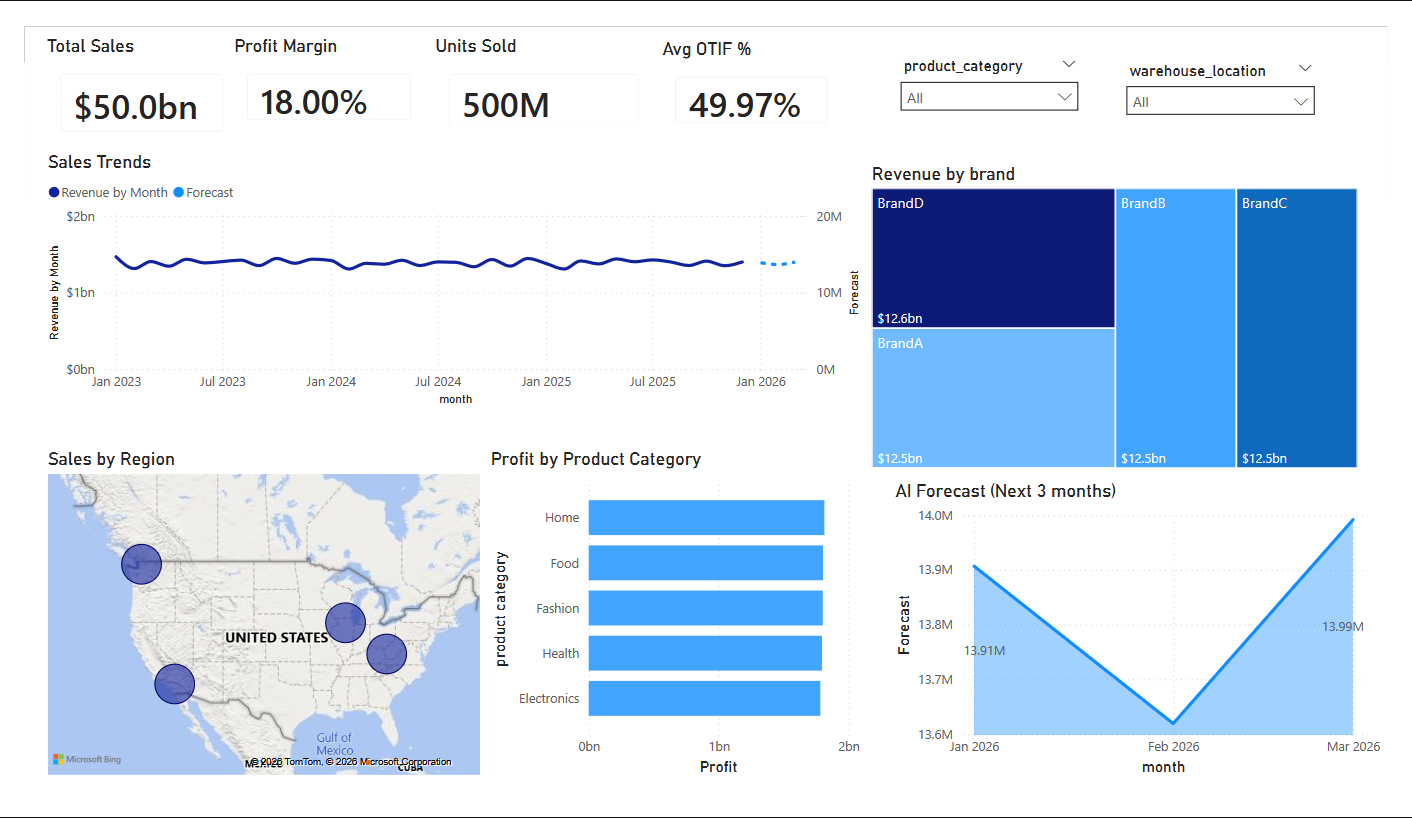
\includegraphics[width=0.95\textwidth]{executive_overview.PNG}
\caption{Executive Summary Dashboard}
\label{fig:dashboard_exec}
\end{figure}

\begin{figure}[H]
\centering
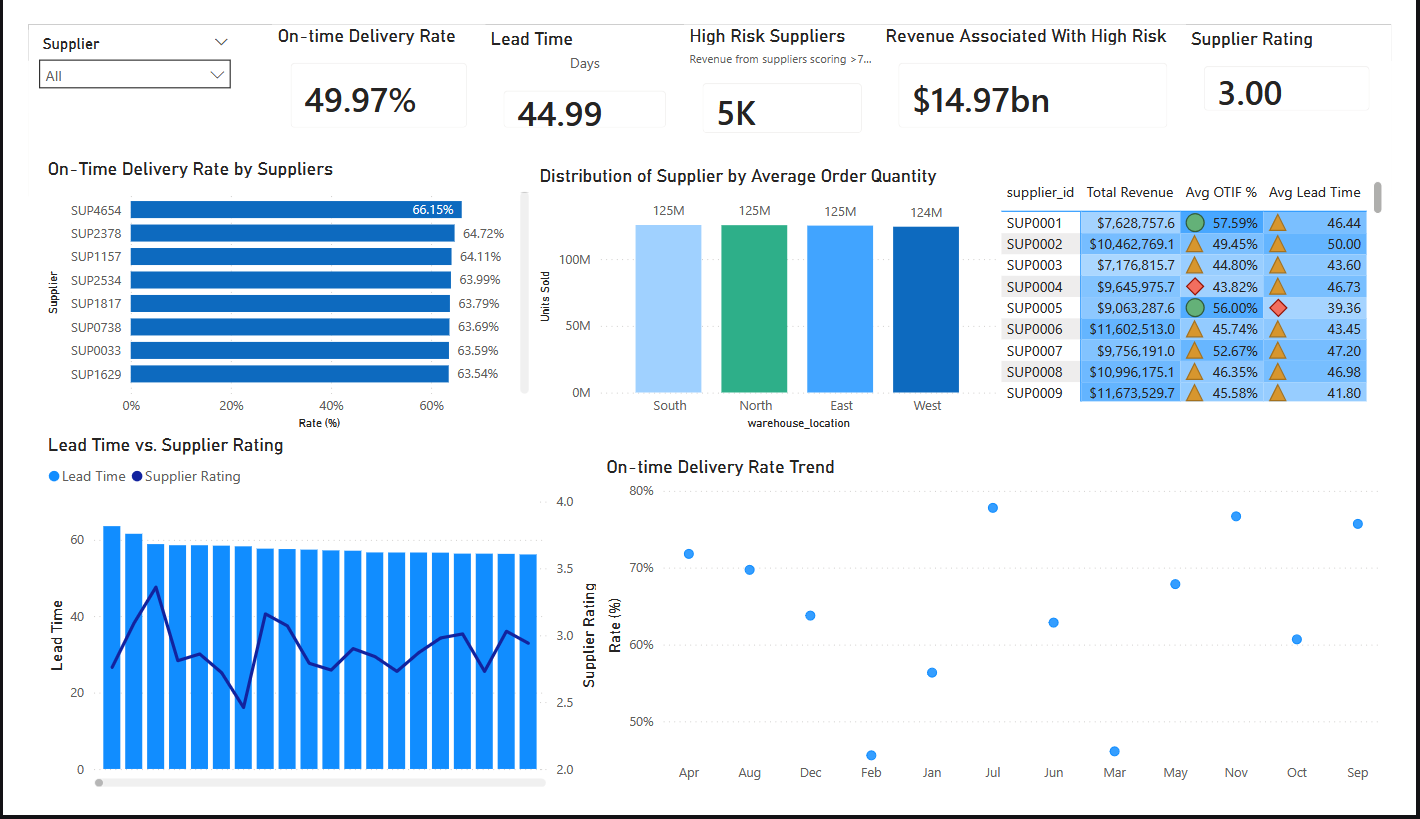
\includegraphics[width=0.95\textwidth]{supplier_performance.PNG}
\caption{Supplier Performance Dashboard}
\label{fig:dashboard_supplier}
\end{figure}

\begin{figure}[H]
\centering
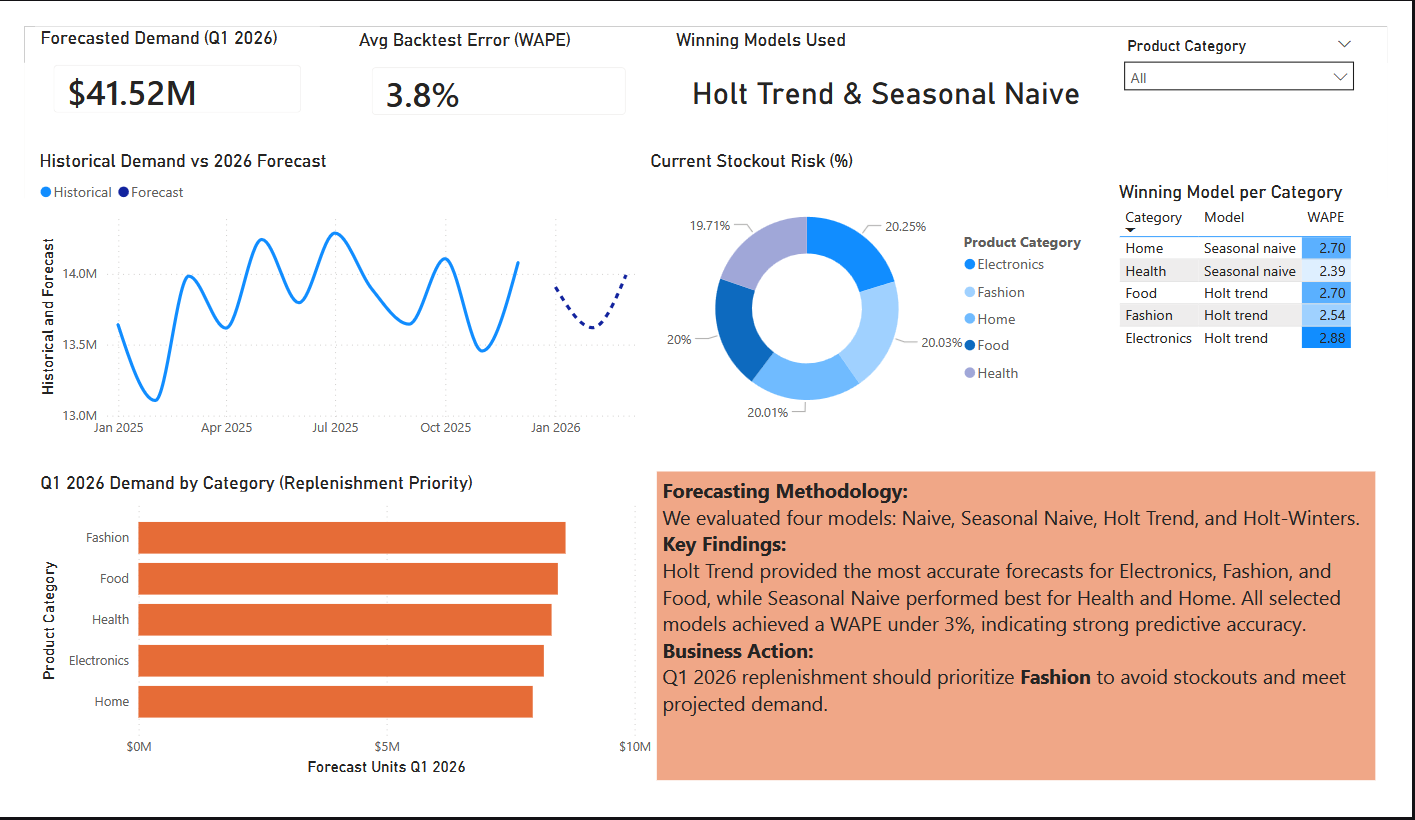
\includegraphics[width=0.95\textwidth]{demand_forecast.PNG}
\caption{Demand Forecasting Dashboard}
\label{fig:dashboard_forecast}
\end{figure}

\end{document}